In diesem Grundlagenkapitel werden alle wichtigen theoretischen Konzepte von Kanalkodierung und im speziellen zu Turbo-Kodes erklärt, um die Implementation in C- beziehungsweise R-Code, das in Kapitel \ref{cha:implementation} erläutert wird, zu verstehen. Die Notation und der Inhalt orientiert sich an dem Buch von Schönfeld \cite{schoenfeld2012informations}.

\section{Kanäle}
\label{sec:channels}
Um Nachrichten an den gewünschten Empfänger zu transportieren, können verschiedene Übertragungsmediums verwendet werden, wie zum Beispiel Kupferkabel oder Funkwellen. Jedes dieser hat spezielle Eigenschaften und Charakteristiken. Damit dieses mit einem Computerprogramm simuliert werden kann, muss ein Modell geschaffen werden, das einen solchen Übertragungskanal bestmöglich abbildet. Dieses Modell bildet alle Störungen und Dämpfungen ab, die während der Übertragung passieren können. Als ein gut geeignetes Modell stellte sich das Überlagern des Signals mit dem \emph{Additiv Weißes Gaußsches Rauschen} (AWGR) heraus \cite[81]{schoenfeld2012informations}. Dieses Rauschen wird folgenderweiße berechnet:

\begin{equation}
E_s = \frac{1}{L} \displaystyle\sum_{i=0}^{L-1} |x[i]|^2; \quad L = length(x)
\label{eq:power}
\end{equation}

In der Formel \ref{eq:power} wird zuerst die Länge der Nachricht ($x$ ist ein Vektor) berechnet, um im Anschluss über alle Bits zu iterieren und die Summe der Quadrate des Signals zu berechnen. Diese Summe wird dann noch durch die Länge dividiert, um die Leistung je Bit zu erhalten.

\begin{equation}
noise = \sqrt{\frac{E_s}{10^{dB/10}}} * randn(1,L)
\label{eq:noise}
\end{equation}

Das Signal/Rausch-Verhältnis muss zuerst vom Dezibel-Bereich in den Linearen umgerechnet, wie im Nenner der Wurzel in der Gleichung \ref{eq:noise} zu sehen ist.
Zur Berechnung des Rauschens werden $L$ Zufallszahlen zwischen 0 und 1 erzeugt und diese mit dem Wurzelergebnis multipliziert. 

\begin{equation}
y = x + noise
\label{eq:noisySignal}
\end{equation}

Danach wird einfach das Rauschen mit dem Originalsignal überlagert, um das verrauschte Signal zu erhalten. Dieses stellt nun den simulierten Übertragungskanal dar, die Stärke der Störung ist mittels der $dB$-Variable zu beeinflussen \cite{AWGN}.

\section{Kanalkodierung}
\label{sec:channelcoding}

\begin{figure}[t]
\centering
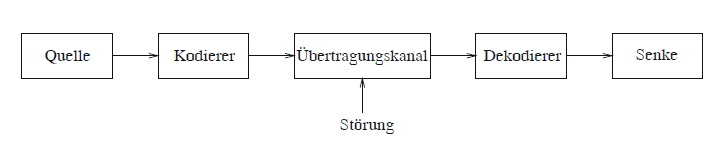
\includegraphics[width=\ScaleIfNeeded]{pictures/Channelmodel}
\caption{Modell der Nachrichtenübertragung, Quelle: \cite[10]{schoenfeld2012informations}}
\label{pic:channelmodel}
\end{figure}

In der Abbildung \ref{pic:channelmodel} ist ein generelles Modell der Nachrichtenübertragung dargestellt, das den Weg einer Nachricht zeigt. Nachdem der Sender (Quelle) die Nachricht durch den Quellenkodierer und Kanalkodierer geschickt hat, gelangt das Kanalwort auf den Übertragungskanal. Dort stören äußere Einflüsse das Signale und verändern es. Beim Empfänger wird versucht, die Nachricht wieder zu dekodieren und die Originalnachricht zu erhalten.

Das Ziel der Kanalkodierung dabei ist den Quellenkodewörtern Redundanz hinzuzufügen, um nach einer fehlerhaften Übertragung über das Übertragungsmedium, die Ausgangsnachricht wieder rekonstruieren zu können. Dabei können Fehler erkannt und im Bestem Fall sogar komplett korrigiert werden.

\subsection{Zweites SHANNONsches Kodierungstheorem}
\label{sec:shannonTheorem}
Auf dem Übertragungskanal wird die zu übertragende Information zu einer bestimmen Wahrscheinlichkeit verfälscht. Durch die Kanalkodierung können Fehler bis zu einem bestimmten Grad korrigiert werden, jedoch bleiben Fehler mit einer bestimmten Restwahrscheinlichkeit.

SHANNON\footnote{Wurde nach Claude Elwood Shannon und Ralph Hartley benannt.} hat mit seinem zweitem Theorem bewiesen, dass es theoretisch möglich ist eine Kanalkodierung zu finden, welche die Restfehlerwahrscheinlichkeit beliebig klein halten kann. Allerdings nur unter der Bedingung, dass der Sender weniger Kodewörter erzeugt, als der Kanaldekodierer beim Empfänger verarbeiten kann. Bereits 1948 erkannte SHANNON eine Grenze, die sogenannte SHANNON-Grenze, welche eine Grenze des Signal/Rausch-Verhältnisses, im Bezug auf die hinzugefügte Redundanz und der erreichbaren Restfehlerwahrscheinlichkeit darstellt. Somit wurde ein Ziel gesteckt mit einer geeigneten Kodierung dieser Grenze möglichst nahe zu kommen \cite[125 f.]{schoenfeld2012informations}.

Ein großer Schritt in Richtung dieser SHANNON-Grenze war im Jahre 1993 die Vorstellung der Turbo-Kodes. Mit denen war es erstmals möglich sehr nahe dieser Grenze zu kommen.

\subsection{Prinzipien der Fehlerkorrektur}
\label{sec:principlesMistakesCorrection}
Die hinzugefügte Redundanz kann auf ganz unterschiedliche Weisen erfolgen. Grundsätzlich gibt es 2 Möglichkeiten diese dem Quellenkodewort hinzuzufügen:

\begin{itemize}
\item Wiederholung der Nachricht
\item Rekonstruktion der Nachricht
\end{itemize}

Bei der ersten Möglichkeit fordert der Empfänger die Nachricht erneut an, wenn er bemerkt, dass die Nachricht nicht korrekt übertragen wurde. Den Fehler erkennen kann er durch Kontrollstellen in der Nachricht, zum Beispiel von Paritätsbits. Bei der zweiten Möglichkeit dient die hinzugefügte Redundanz nicht nur zur Erkennung der Fehler, sondern auch als Hilfe zur Rekonstruktion der Originalnachricht. Natürlicherweise muss die Redundanz größer sein, als bei der ersten Methode, die nur Fehler erkennt.

Es wird vorausgesetzt, dass die Wahrscheinlichkeit von Einzelfehlern größer ist, als das Auftreten von Bündelfehlern, also mehrere Fehler hintereinander. Jede Kodierung hat seine Grenze, deswegen kann auch der Beste Dekodierer nicht unendliche viele Fehler korrigieren. Zur Rekonstruktion des Kodewortes wird die \emph{Maximum-Likelihood-Methode} verwendet. Dabei wird das Kodewort gesucht, das einem existierendem, realistischen Wort am nähesten liegt. Dadurch liefert der Dekodierer immer ein Kodewort, das die geringste Distanz zum gesendeten Kodewort aufweist. Das bedeutet jedoch nicht, dass es unbedingt die richtige Nachricht sein muss. Der Berechnungsaufwand dieser Methode steigt allerdings mit der Länge der Nachricht enorm \cite[126-129]{schoenfeld2012informations}. 

\subsection{Verwendete Notation}
\label{sec:notation}
In den folgenden Kapiteln werden immer wieder Variablen verwendet, die aber nicht bei der konkreten Formel eingeführt werden. Deshalb wird in diesem Kapitel einmal die Variablen eingeführt und dann immer verwendet Bei diesen Definition werden immer Kodewörter mit dem Alphabet ${0,1}$ verwendet, da dieser Fall am meisten Bedeutung hat.

Nachrichten werden zuerst mit dem Quellenkodierer in eine möglichst redundanzfreie Form gebracht, um die verwendeten Bits möglichst gut auszunutzen. Diese Kodewörter werden als Quellenkodewörter bezeichnet und sind folgenderweise definiert:

\begin{t_def}
Ein Wort $a^* \in {0,1}^l$ wird als Quellenkodewort der Länge $l$ bezeichnet.
\end{t_def}

Im Anschluss wird Redundanz den Quellenkodewörtern durch den Kanalkodierer hinzugefügt, das resultierende Kodewort sieht folgenderweise aus:

\begin{t_def}
Ein Wort $a \in {0,1}^n$ wird als Kanalkodewort der Länge $n$ bezeichnet.
\end{t_def} 

Durch das hinzufügen von Redundanz ergeben sich $k = n - l$ redundante Stellen. Diese werden zur Fehlererkennung und Fehlerkorrektur bei der Dekodierung verwendet.

Zum Beispiel erzeugt ein Quellenkodierer Nachrichten der Länge $l=2$, $a^*_{1}=(00),a^*_{2}=(01),a^*_{3}=(10),a^*_{4}=(11)$. Danach fügt der Kanalkodierer eine redundante Stelle hinzu $k=1$, also haben die Nachrichten dann eine Länge von $n=3$. Sie könnten folgenderweise aussehen, $a_{1}=(001),a_{2}=(010),a_{3}=(100),a_{4}=(110)$.

\subsection{Kenngrößen von Kanalkodes}
\label{sec:channelParameters}
Für die Betrachtung von verschiedenen Kanalkodierungen ist es wichtig Unterscheidungsmerkmale zu finden. Diese werden in diesem Kapitel eingeführt. Dazu wird als erstes in Kapitel \ref{sec:hammingDistance} die Distanz zwischen zwei Kodewörtern erklärt, um im Anschluss in Kapitel \ref{sec:hammingWeight} das Gewicht eines Wortes berechnen zu können. Am Schluss in Kapitel \ref{sec:codeRate} wird noch der Begriff der Kode-Rate eingeführt.

\subsubsection{Hamming-Distanz}
\label{sec:hammingDistance}
Damit durch einzelne Fehler auf dem Übertragungskanal, nicht eine anderes existierende Nachricht produziert wird, sollen Kodewörter angestrebt werden, die sich möglichst weit unterscheiden. Eine wichtige Kenngröße dabei ist der Abstand zwischen zwei Kodewörtern:

\begin{t_def}
Anzahl der Stellen, in denen sich 2 Kodewörter $a_i$ und $a_j$ unterscheiden. Die Zahl nennt man die\emph{Hamming-Distanz} zwischen den beiden Wörtern.
\end{t_def} 
 
\begin{equation}
d(a_i,a_j) = \sum^{n}_{g=1} (u_{ig} \oplus u_{jg})
\label{eq:hammingDistance}
\end{equation}

Diese lässt sich bei Binärkodes mit der Formel \ref{eq:hammingDistance} berechnen, dabei wird einfach gezählt, wie viele Stellen sich unterscheiden. Interessant ist der kleinste Unterschied zwischen zwei Kodewörtern, die Zahl wird \emph{minimale Hamming-Distanz} $d_{min}$ genannt.

Ein Kode der alle Verfälschungen $\leq f_e$ erkennen kann, muss eine \emph{minimale Hamming-Distanz} von 

\begin{equation}
d_{min} = f_e + 1
\end{equation}

besitzen. Mit $f_e$ wird Grad der Fehlererkennung genannt. Die Anzahl der korrigierbaren Fehler $f_k$ lässt sich folgenderweise berechnen:

\begin{equation}
f_k = \frac{d_{min}-1}{2}
\end{equation}

Damit nun Fehler erkannt und korrigiert werden können, muss die \emph{minimale Hamming-Distanz} mindestens folgende Gleichung erfüllen \cite[132 f.]{schoenfeld2012informations}:

\begin{equation}
d_{min} = f_e + f_k + 1
\end{equation} 

\subsubsection{Hamming-Gewicht}
\label{sec:hammingWeight}

\subsubsection{Kode-Rate}
\label{sec:codeRate}

\section{Turbo-Kodes}
\label{sec:turboCodes}